% ==============================================================================
% INIZIO DISPENSA: PROGETTAZIONE DI UN DATA WAREHOUSE
% ==============================================================================

\chapter{Progettazione di un Data Warehouse}

La decisione di un'azienda di dotarsi di un sistema di data warehouse per la business intelligence (o per il supporto strategico e decisionale) è un passo fondamentale. Sebbene oggi sia una scelta diffusa non solo tra le grandi aziende ma anche in contesti di medie dimensioni, l'adozione di questi strumenti non risolve automaticamente tutti i problemi aziendali. L'obiettivo principale è ottenere evidenze di tipo \textit{data-driven} sullo stato dell'azienda, ma il successo del sistema dipende da una corretta progettazione, dalla qualità dei dati e dalla collaborazione tra attori con visioni differenti.

Un'architettura tipica per il supporto decisionale è composta da almeno due livelli separati: il livello delle sorgenti (sistemi transazionali/operazionali) e il livello di organizzazione delle informazioni per le analisi (il data warehouse vero e proprio). Mantenere separati i sistemi operazionali dai sistemi decisionali è cruciale per ragioni di efficienza e prestazioni. Spesso si adotta un'architettura a tre livelli, introducendo un livello intermedio di alimentazione (con una \textit{staging area}) in cui avvengono i processi di ETL (Estrazione, Trasformazione e Caricamento).

\section{Fattori di Rischio e Approcci alla Progettazione}

\subsection{Fattori di rischio}
La realizzazione di un data warehouse comporta dei rischi intrinseci dovuti alla necessità di far comunicare due "mondi" separati:
\begin{itemize}
    \item \textbf{Gestione "politica" del progetto e collaborazione:} Da un lato vi sono gli amministratori dei DBMS tradizionali (sistemi informativi), abituati a logiche dove ogni dato deve essere memorizzato al massimo livello di dettaglio senza ridondanze. Dall'altro vi sono gli utenti di business (decision maker), che necessitano di dati aggregati per l'esplorazione e non conoscono a priori il livello di dettaglio di cui avranno bisogno. L'accettazione del sistema da parte degli utenti finali e la collaborazione dei "detentori" dell'informazione è vitale.
    \item \textbf{Aspettative elevate:} Esiste il rischio che gli utenti vedano il data warehouse come la panacea di tutti i problemi aziendali. Il sistema sarà invece efficace se e solo se nelle sorgenti esistono i dati corretti per alimentare le analisi richieste.
    \item \textbf{Qualità dei dati e processi di partenza:} I dati operazionali possono essere incompleti o inaffidabili, e i processi aziendali potrebbero non essere integrati o ottimizzati, compromettendo la base stessa su cui si fonda il supporto decisionale.
\end{itemize}

\subsection{Approcci: Top-Down vs Bottom-Up}
Per realizzare un data warehouse si possono seguire due approcci principali:

\subsubsection{Approccio Top-Down}
Consiste nel realizzare un data warehouse che fornisca fin da subito una visione globale e completa di tutti i dati aziendali. Si ha in mente l'intero spettro delle analisi necessarie per tutta l'azienda e si progetta il sistema complessivo.
\begin{itemize}
    \item \textbf{Svantaggi:} Richiede un costo economico e temporale molto significativo, con analisi e progettazioni estremamente complesse. Ad esempio, pensare di creare con un approccio top-down un data warehouse per l'intero Politecnico di Torino (con dipartimenti, amministrazione, decine di migliaia di studenti e personale) è un progetto troppo ambizioso e di lungo termine.
    \item \textbf{Utilizzo:} In contesti medio-grandi è generalmente sconsigliato a causa della necessità di una visione troppo estesa.
\end{itemize}

\subsubsection{Approccio Bottom-Up}
Consiste in una realizzazione incrementale. Si parte da un settore aziendale specifico (un problema più circoscritto, seppur grande) e si realizza un \textbf{data mart}, ovvero un piccolo data warehouse specializzato per quel contesto (es. gestione del magazzino, gestione delle vendite).
\begin{itemize}
    \item \textbf{Vantaggi:} Il costo e il tempo di consegna sono contenuti. I vari data mart, che inizialmente possono anche essere indipendenti, verranno poi aggregati e integrati in fasi successive per formare il data warehouse aziendale completo.
\end{itemize}

\begin{figure}[H]
    \centering
    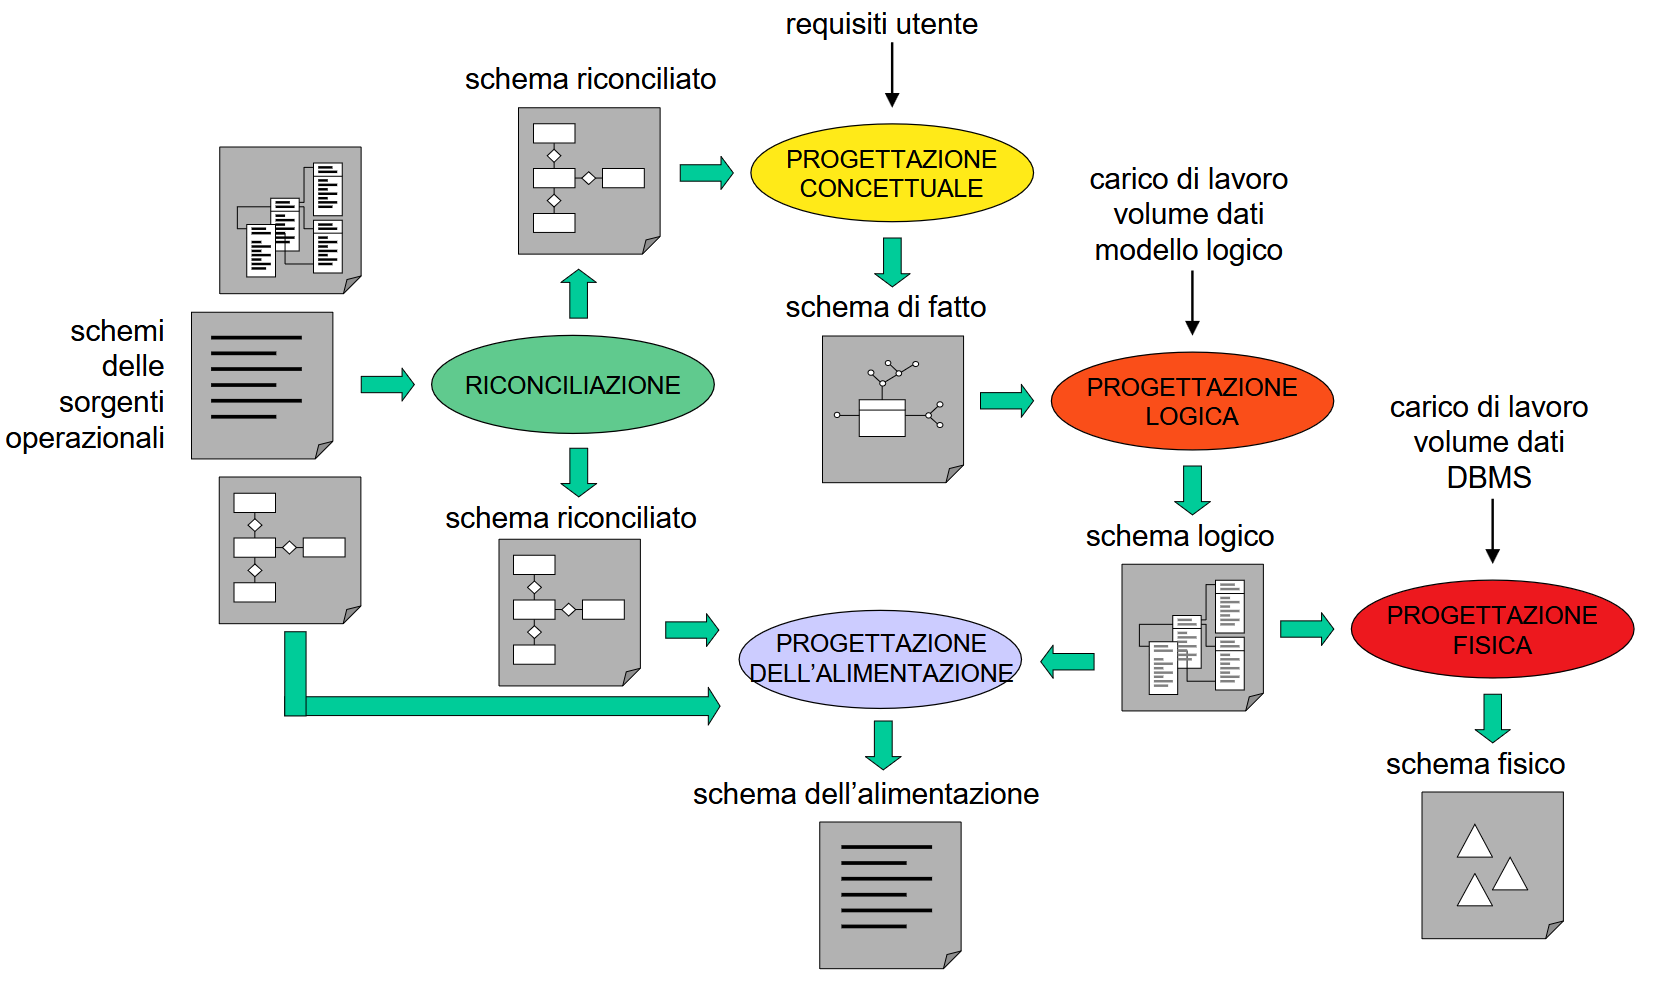
\includegraphics[width=0.75\textwidth]{capitoli/03_Data warehouse_progettazione concettuale e logica/images/approccio_bottom_up.png}
    \caption{Approccio Bottom-Up: si parte da un data mart specifico e si procede all'integrazione con altri data mart per formare il data warehouse completo.}
\end{figure}

\section{Analisi dei Requisiti}

Il processo di realizzazione di un data mart (approccio bottom-up) inizia sempre dall'analisi dei requisiti. Si tratta di comprendere quali sono le analisi di interesse per gli attori di business (che variano a seconda del ruolo, es. direttore vendite vs capo del personale) e identificare i dati necessari per supportarle. 

La raccolta dei requisiti avviene tipicamente tramite \textbf{interviste} che coinvolgono sia i \textit{business users} (utilizzatori finali) sia gli amministratori del sistema informativo. Di norma, il primo data mart sviluppato riguarda un settore strategico dell'azienda per dimostrare fin da subito l'efficacia del progetto.

La progettazione si basa su tre pilastri (pillar) fortemente interconnessi:
\begin{enumerate}
    \item \textbf{Tecnologia:} Quale DBMS usare, spazio di archiviazione, livello di affidabilità.
    \item \textbf{Dati:} Quali dati servono, se sono presenti nelle sorgenti interne o se vanno integrati con fonti esterne, e come effettuare l'integrazione.
    \item \textbf{Applicazioni:} Che tipo di applicativo utilizzerà l'utente finale (dashboard interattiva, algoritmi predittivi, soluzioni agentiche basate su LLM/RAG). La tecnologia scelta deve supportare l'applicazione desiderata.
\end{enumerate}

I requisiti si dividono in due grandi categorie: applicativi e strutturali.

\subsection{Requisiti Applicativi}
Definiscono il "che cosa" si vuole analizzare.
\begin{itemize}
    \item \textbf{Descrizione degli eventi di interesse (Fatti):} Un fatto rappresenta una categoria di eventi aziendali (es. reclami, quantità venduta, giacenze di magazzino). È caratterizzato da coordinate di analisi (dimensioni) e da indicatori numerici (misure o KPI).
    \item \textbf{Carico di lavoro:} Quali e quanti attori accedono al sistema, la frequenza di generazione dei report, il numero di sessioni in contemporanea. Queste informazioni permettono di dimensionare opportunamente il sistema.
\end{itemize}

\subsection{Requisiti Strutturali}
Riguardano l'infrastruttura e i vincoli operativi.
\begin{itemize}
    \item \textbf{Periodicità dell'alimentazione:} Il data warehouse necessita di un caricamento periodico (ETL). Solitamente avviene nelle ore notturne, quando il carico dei sistemi informativi e del data warehouse è minimo.
    \item \textbf{Spazio disponibile:} Sia per i dati grezzi che per strutture accessorie necessarie a velocizzare le interrogazioni (indici, viste materializzate).
    \item \textbf{Tipo di architettura:} A due o tre livelli, e definizione se i data mart saranno dipendenti (condividono dimensioni di analisi) o indipendenti.
\end{itemize}

\section{Progettazione Concettuale: Dimensional Fact Model (DFM)}

Dopo aver raccolto i requisiti (e aver definito uno schema riconciliato delle sorgenti nel caso di sistemi informativi eterogenei), si passa alla progettazione concettuale. In questo ambito, il \textbf{modello Entità-Relazione (ER) non è adatto}.
Il modello ER nasce per i DBMS operazionali: il suo scopo è normalizzare i dati per evitare ridondanze e prevenire anomalie di aggiornamento. Tuttavia, uno schema normalizzato frammenta l'informazione; per ricostruirla in fase di interrogazione analitica (su milioni di record) sarebbero necessarie numerose operazioni di \texttt{JOIN}, rendendo il sistema inefficiente.

Nel data warehouse \textbf{rinunciamo alla normalizzazione e accettiamo la ridondanza} per ottenere query efficienti. Il modello concettuale di riferimento è il \textbf{Dimensional Fact Model (DFM)}, introdotto da Golfarelli e Rizzi, che offre una rappresentazione grafica basata su fatti, dimensioni e misure.

\subsection{Elementi Base del DFM}

\begin{itemize}
    \item \textbf{Fatto:} Modella un insieme di eventi di interesse (es. vendite). Nel DFM è rappresentato dal nodo centrale. Solitamente, in un modello ER equivalente, il fatto rappresenta una relazione molti-a-molti (ennaria) tra tutte le dimensioni coinvolte (es. lo stesso prodotto può essere venduto in più negozi e in più date).
    \item \textbf{Dimensione:} Descrive le coordinate di analisi di un fatto (es. Negozio, Prodotto, Data). Le dimensioni sono tendenzialmente ortogonali tra loro.
    \item \textbf{Misura (o Metrica):} Una proprietà numerica associata al fatto, oggetto di operazioni di aggregazione (es. quantità venduta, incasso, numero di clienti).
    \item \textbf{Gerarchia:} Sulle dimensioni è possibile definire delle gerarchie (es. Data $\rightarrow$ Mese $\rightarrow$ Trimestre $\rightarrow$ Anno). Esse rappresentano generalizzazioni di concetti e modellano una \textbf{dipendenza funzionale} (relazione 1:N). 
\end{itemize}

\subsubsection{Le Gerarchie e le Dipendenze Funzionali}
Nel DFM, un arco in una gerarchia rappresenta una dipendenza funzionale, ovvero, dato l'attributo di partenza, esiste \textit{uno e un solo} valore per l'attributo di destinazione. 
L'arco va tracciato solo verso l'attributo meno generale immediatamente successivo. Ad esempio, esiste una dipendenza funzionale tra \textit{Data} e \textit{Anno}, ma l'arco viene disegnato da \textit{Data} a \textit{Mese}, e da \textit{Mese} a \textit{Trimestre}, e da quest'ultimo ad \textit{Anno}.
Inoltre, non si traccia un arco tra \textit{Giorno della settimana} (lunedì, martedì...) e \textit{Anno}, perché un "lunedì" non appartiene univocamente a un solo anno (non c'è dipendenza funzionale 1:N).

Un'attenzione particolare va posta al concetto temporale nel business: quando si parla di "analisi per mese", si intende quasi sempre il mese in un determinato anno (es. Settembre 2026), distinto dal mese di un altro anno. Se l'obiettivo fosse analizzare tutti i mesi di settembre a prescindere dall'anno, si parlerebbe di "mese dell'anno".

% FIGURA ORIGINALE DA RECUPERARE DALLE SLIDE
% Slide di provenienza: 11
% Tipo: schema
% Descrizione: Rappresentazione grafica di un Dimensional Fact Model (DFM) di base con il fatto Vendita, dimensioni, gerarchie e misure.
% Punto di inserimento: Qui, per mostrare un esempio di schema DFM.
% File da inserire: dfm_base_vendita.png
\begin{figure}[H]
    \centering
    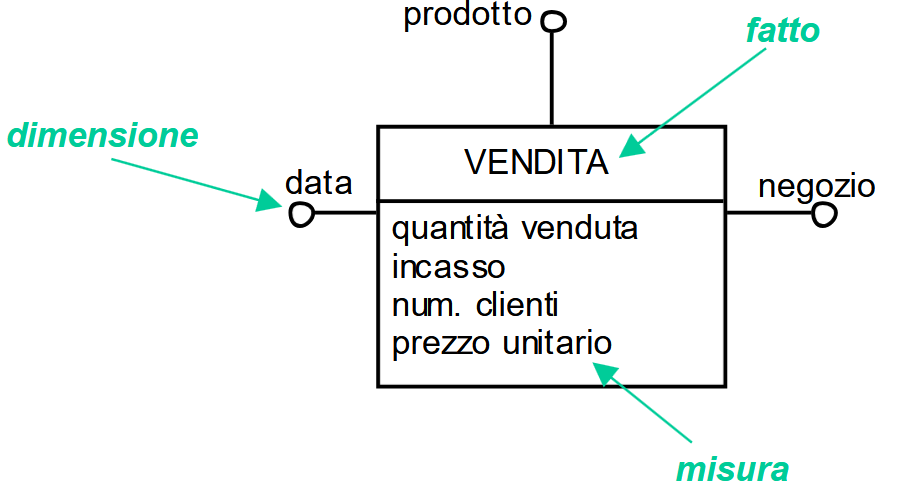
\includegraphics[width=0.6\textwidth]{capitoli/03_Data warehouse_progettazione concettuale e logica/images/dfm_base_vendita.png}
    \caption{Esempio di Dimensional Fact Model per le vendite, con dimensioni (Negozio, Prodotto, Data), gerarchie (es. Negozio $\rightarrow$ Città) e misure (Qta, Incasso).}
    \label{fig:dfm-base}
\end{figure}

\subsection{Confronto: DFM vs Modello ER}
Se traducessimo un fatto in un modello ER, esso diventerebbe un'entità associativa centrale che collega con relazioni N:1 le varie entità dimensionali, le quali a loro volta si esploderebbero a cascata a causa delle dipendenze funzionali (gerarchie) in una miriade di tabelle (forma normale). Il DFM "collassa" visivamente e logicamente queste gerarchie.

% FIGURA ORIGINALE DA RECUPERARE DALLE SLIDE
% Slide di provenienza: 14
% Tipo: diagramma
% Descrizione: Confronto tra uno schema DFM e il corrispondente modello ER altamente normalizzato.
% Punto di inserimento: Qui, a supporto della spiegazione sul superamento del modello ER.
% File da inserire: dfm_vs_er.png
\begin{figure}[H]
    \centering
    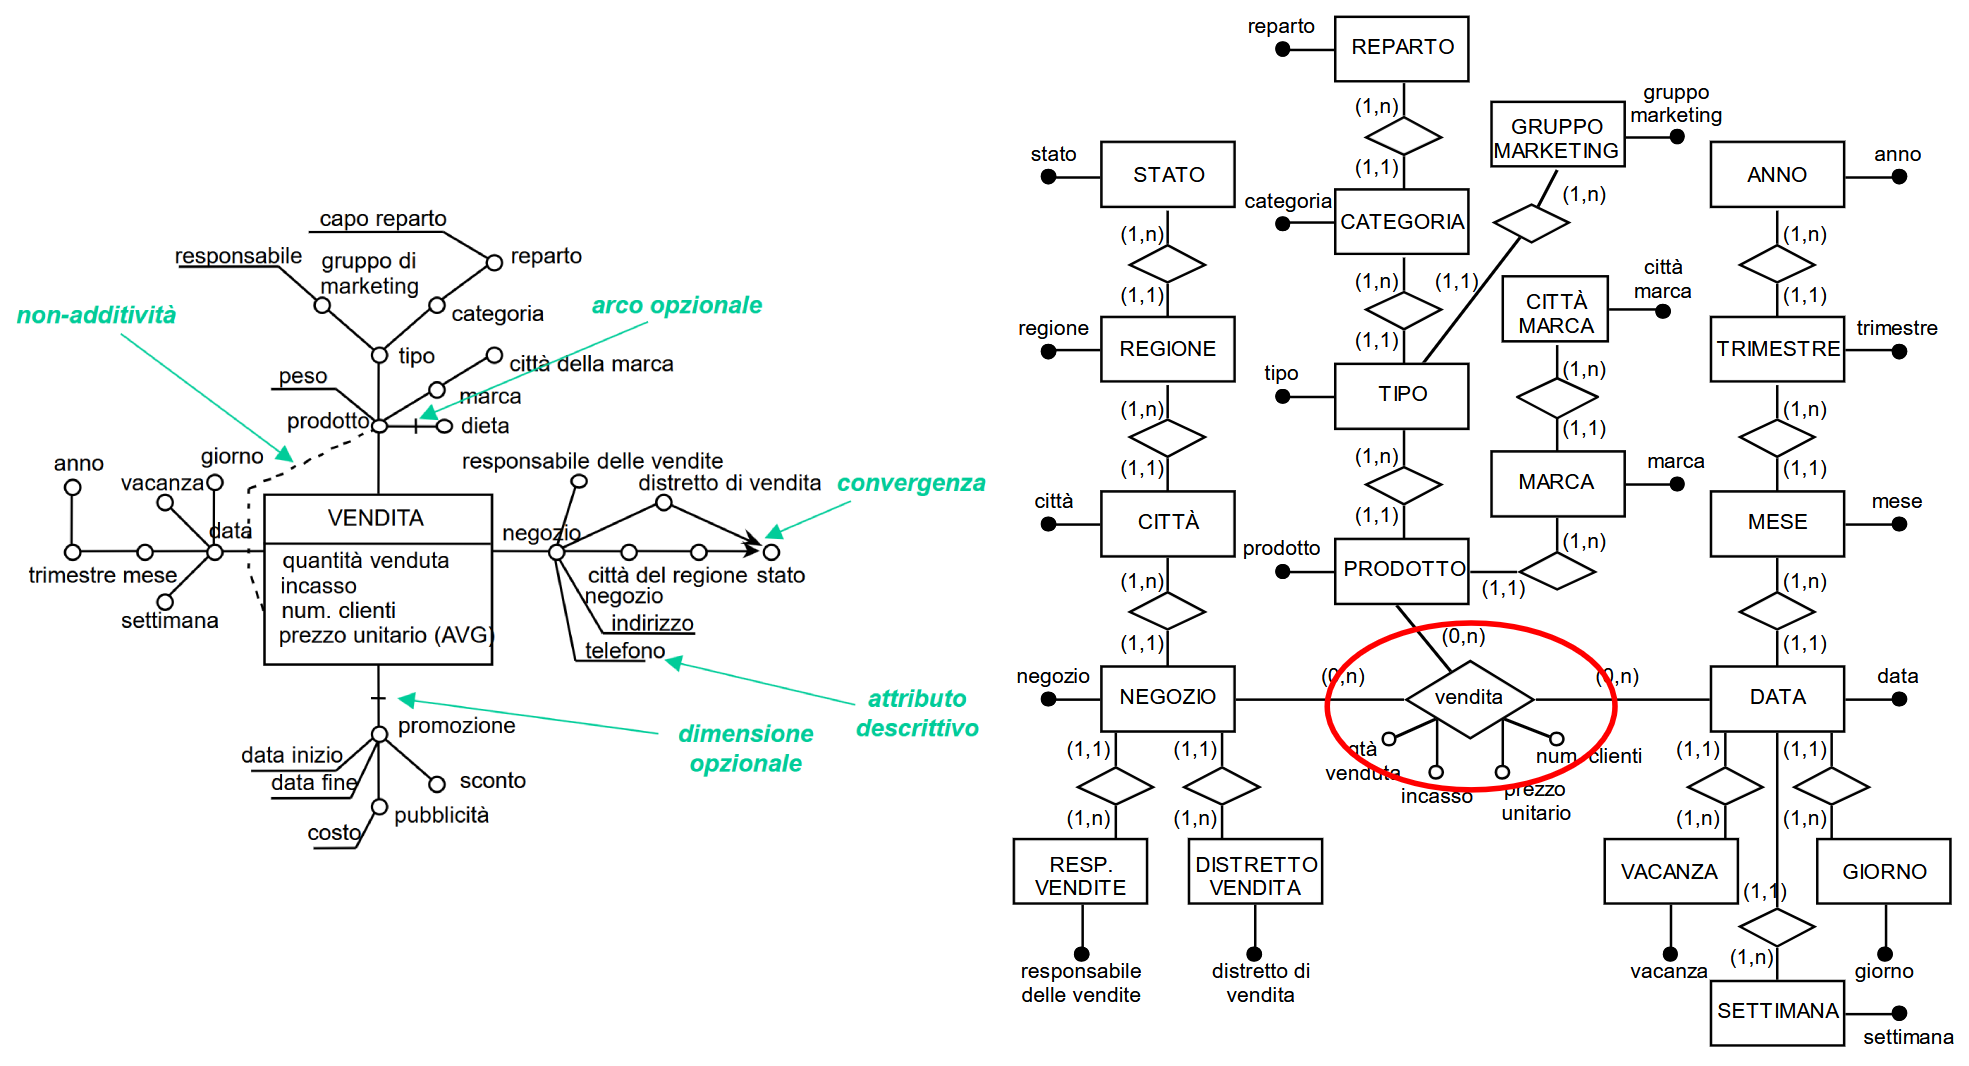
\includegraphics[width=0.95\textwidth]{capitoli/03_Data warehouse_progettazione concettuale e logica/images/dfm_vs_er.png}
    \caption{Confronto tra la notazione compatta del DFM (a sinistra) e la complessità di un modello ER equivalente (a destra) dove tutte le dipendenze funzionali sono esplicitate in tabelle separate.}
    \label{fig:dfm-vs-er}
\end{figure}

\section{Misure e Operatori di Aggregazione}

Il processo tipico in un data warehouse è l'analisi a diversi livelli di dettaglio, che corrisponde in SQL all'applicazione della clausola \texttt{GROUP BY} navigando lungo le gerarchie. È fondamentale capire quali misure possono essere aggregate e come.

\subsection{Classificazione delle Misure}
Le metriche si dividono in tre categorie in base alla loro additività (la capacità di essere sommate lungo le dimensioni, specialmente il tempo):

\begin{enumerate}
    \item \textbf{Misure di flusso:} Possono essere valutate cumulativamente alla fine di un periodo di tempo. Sono \textbf{sempre additive} lungo tutte le dimensioni.
    \begin{itemize}
        \item \textit{Esempi:} Quantità di prodotti venduti, importo incassato. Se vendo 10 oggetti oggi e 20 domani, in totale ho venduto 30 oggetti.
    \end{itemize}
    \item \textbf{Misure di livello:} Rappresentano un'istantanea (snapshot) di un fenomeno in un preciso istante di tempo. \textbf{Non sono additive lungo la dimensione temporale}.
    \begin{itemize}
        \item \textit{Esempi:} Giacenza di magazzino, saldo del conto corrente. Se oggi ho 100€ sul conto e domani ho 100€, la somma 200€ non ha alcun significato; il valore "fotografa" lo stato attuale. Tuttavia, \textit{possono} essere additive lungo lo spazio (es. somma delle giacenze di tre magazzini diversi nello stesso istante).
    \end{itemize}
    \item \textbf{Misure unitarie:} Valutate in specifici istanti ed espresse in termini relativi. \textbf{Non sono additive} lungo nessuna dimensione.
    \begin{itemize}
        \item \textit{Esempio:} Prezzo unitario di un prodotto.
    \end{itemize}
\end{enumerate}

Un'ulteriore eccezione all'additività si ha quando l'aggregazione su una dimensione genera duplicati di conteggio. Ad esempio, la metrica \textit{Numero Clienti} calcolata come numero di scontrini: è sommabile nel tempo, ma \textbf{non è additiva rispetto ai Prodotti}. Poiché uno stesso cliente può comprare più prodotti in uno stesso scontrino, aggregare i clienti per prodotto porterebbe a contare la stessa persona più volte (overlap). Sul DFM questa non-additività va esplicitata graficamente.

\subsection{Operatori di Aggregazione}
A seconda di come è possibile calcolare aggregazioni partendo da dati già pre-aggregati a un livello di dettaglio maggiore, gli operatori si classificano in:

\begin{itemize}
    \item \textbf{Distributivi:} Il calcolo finale può sfruttare risultati aggregati intermedi. (es. \texttt{SUM}, \texttt{MIN}, \texttt{MAX}). 
    \textit{Esempio:} Per calcolare le vendite annuali, posso sommare i parziali delle vendite trimestrali già calcolati. Questo abbassa drasticamente i tempi di calcolo.
    \item \textbf{Algebrici:} Il risultato intermedio da solo non basta, ma è possibile calcolarlo se affiancato da misure di supporto. (es. \texttt{AVG}).
    \textit{Motivazione:} La media delle medie è matematicamente scorretta. Per aggregare una media a un livello superiore, il data warehouse non dovrebbe memorizzare la "media" come metrica secca, ma memorizzare le metriche di base che la compongono (es. l'incasso e il numero di prodotti) per ricalcolarla in SQL come \texttt{SUM(Incasso) / SUM(Num\_Prodotti)}.
    \item \textbf{Olistici:} Non è possibile sfruttare alcun aggregato parziale; è necessario ricalcolare la funzione partendo dai dati originali di massimo dettaglio. (es. Moda, Mediana).
\end{itemize}

\section{Costrutti Avanzati nel DFM}

La modellazione concettuale deve saper gestire casi della realtà aziendale più complessi.

\subsection{Attributi Descrittivi e Gerarchie Condivise}
\begin{itemize}
    \item \textbf{Attributi descrittivi:} Sono caratteristiche associate a una dimensione su cui però \textit{non si fanno aggregazioni} (es. Indirizzo, Telefono del negozio). Si rappresentano graficamente con una linea semplice (senza cerchio).
    \item \textbf{Gerarchia Condivisa:} Spesso una stessa dimensione assume "ruoli" multipli nello stesso fatto. L'esempio classico è il traffico telefonico: una chiamata ha un \textit{Numero Chiamante} e un \textit{Numero Chiamato}. Entrambi puntano all'entità Numero Telefonico (che possiede una sua gerarchia, es. Distretto, Uso). Nel DFM si tracciano due frecce separate dal Fatto alla dimensione, specificando il ruolo su ciascuna freccia. Altri esempi: aeroporto di partenza e destinazione in un volo; mittente e destinatario in una spedizione o in un bonifico.
\end{itemize}

\subsection{L'Arco Multiplo}
Come abbiamo visto, la gerarchia modella dipendenze funzionali 1:N. Ma cosa succede quando tra due attributi dimensionali esiste una \textbf{relazione Molti-a-Molti}?
Si utilizza l'arco multiplo, rappresentato da due linee convergenti.

\textbf{Casi d'uso:}
\begin{enumerate}
    \item \textbf{Libri e Autori:} Vogliamo analizzare le vendite di libri. Un libro può essere scritto da più autori, un autore scrive più libri. Date le vendite del "Libro X", ad esso è associato un numero indefinito di autori.
    \item \textbf{Ricoveri e Diagnosi:} Un paziente in pronto soccorso può avere un "Gruppo di diagnosi" che racchiude $N$ patologie diverse. Associando il costo del ricovero all'intero gruppo (più specifico) e connettendo il gruppo alla singola diagnosi (tramite arco multiplo), semplifichiamo il calcolo del costo evitando di duplicarlo o distribuirlo in modo arbitrario tra le singole patologie.
\end{enumerate}

L'arco multiplo è obbligatorio quando non si conosce a priori il numero massimo di valori (es. numero di autori di un libro) oppure quando tale numero è grande.

\subsection{L'Attributo Configurazione}
Se abbiamo un attributo multivalore (come l'arco multiplo) ma \textbf{conosciamo a priori i valori ammissibili e questi sono pochi (generalmente $\le 10$)}, possiamo semplificare notevolmente il modello.
Invece di creare un nodo separato e richiedere complessi \texttt{JOIN}, inseriamo nel modello un \textbf{Attributo Configurazione}. 

\textit{Funzionamento:} Si "esplode" l'informazione creando un attributo booleano (Sì/No) per ciascun valore possibile. 
\textit{Esempi:}
\begin{itemize}
    \item Un negozio di videogame che può vendere 4 specifiche tipologie di giochi. Avremo 4 campi booleani nel record del negozio.
    \item Le università e l'elenco dei servizi gratuiti (Wi-Fi, Sale studio, Mensa). Se i servizi mappati sono meno di 10, usiamo una configurazione.
\end{itemize}
Questo costrutto rende le query analitiche molto più semplici, potendo filtrare direttamente con predicati booleani nella clausola \texttt{WHERE}.

% FIGURA ORIGINALE DA RECUPERARE DALLE SLIDE
% Slide di provenienza: 21 e 22
% Tipo: schema
% Descrizione: Esempi di costrutti avanzati del DFM: Arco Multiplo (Libro-Autore) e Attributo Configurazione (Categorie di videogame).
% Punto di inserimento: Qui, per visualizzare le alternative descritte sopra.
% File da inserire: dfm_costrutti_avanzati.png
\begin{figure}[H]
    \centering
    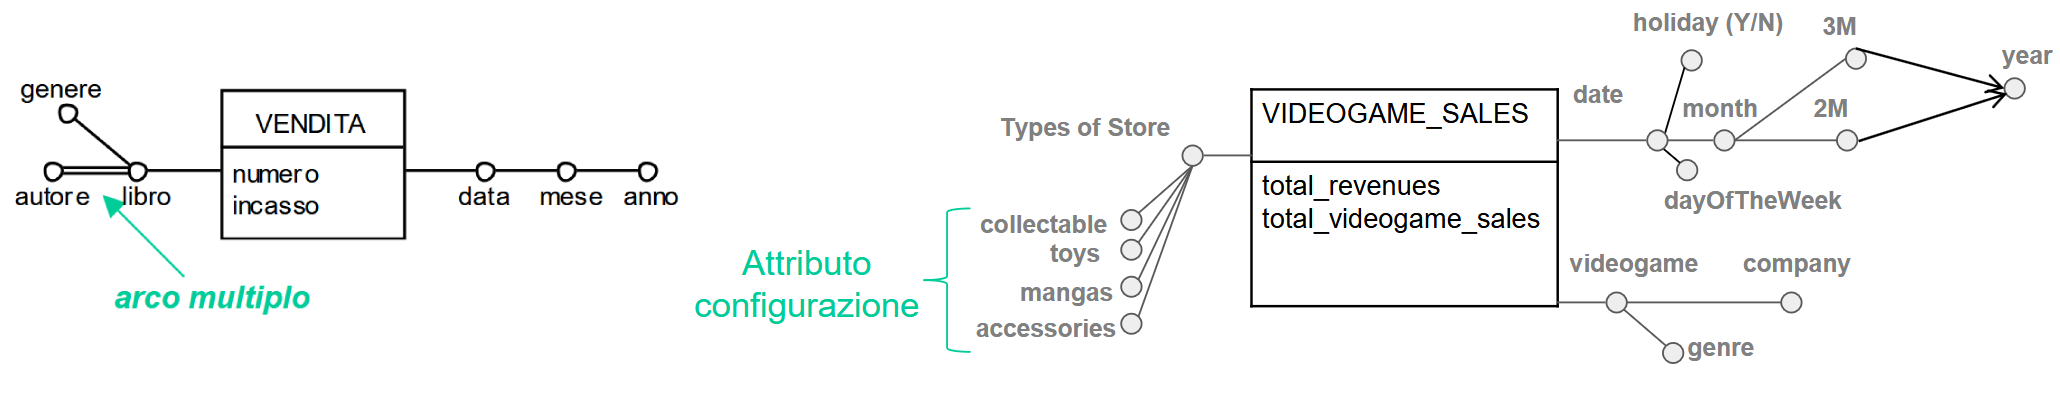
\includegraphics[width=0.9\textwidth]{capitoli/03_Data warehouse_progettazione concettuale e logica/images/dfm_costrutti_avanzati.png}
    \caption{Rappresentazione di un arco multiplo (a sinistra) e di un attributo configurazione (a destra) nel Dimensional Fact Model.}
    \label{fig:dfm-costrutti-avanzati}
\end{figure}

\subsection{Schemi di Fatto Vuoti}
Non tutti i fatti registrano valori monetari o metriche di flusso. Se l'obiettivo è memorizzare \textbf{la pura presenza/verificarsi di un evento}, creiamo uno \textit{schema di fatto vuoto}, ovvero privo di misure.
\textit{Esempio:} La frequenza degli studenti ai corsi. L'evento è caratterizzato dalle dimensioni Studente, Semestre, Corso. Se la tripla esiste nel Data Warehouse, l'evento si è verificato. In questo caso, l'unico operatore di aggregazione applicabile nelle query è il \texttt{COUNT(*)} per contare gli eventi accaduti.

\section{La Rappresentazione del Tempo (Slowly Changing Dimensions)}

Il data warehouse conserva lo storico aziendale. I fatti sono intrinsecamente legati al tempo (dimensione Data), ma anche gli attributi delle altre dimensioni possono subire \textbf{variazioni lente nel tempo} (Slowly Changing Dimensions - SCD), ad esempio un cliente che cambia stato civile, o un prodotto che cambia nome o packaging.
Gestire questi cambiamenti è vitale per non falsare le analisi. Esistono tre modalità (o Tipi) principali:

\subsection{Rappresentazione di Tipo 1 (Sovrascrittura)}
È la fotografia dell'istante attuale. Il valore vecchio viene \textbf{sovrascritto} con quello nuovo.
\begin{itemize}
    \item \textit{Esempio:} Il cliente Mario Rossi si sposa. Lo stato civile viene sovrascritto. Tutti gli acquisti fatti da single figurano ora come fatti da "sposato". Anche un prodotto (es. cereali) che cambia nome, assocerebbe tutte le vendite passate al nuovo nome.
    \item \textit{Problema:} Si perde totalmente la memoria storica e la correlazione tra l'evento temporale (il cambio) e i volumi. In contesti reali è fortemente sconsigliato.
\end{itemize}

\subsection{Rappresentazione di Tipo 2 (Nuova Istanza)}
Per ogni variazione si crea un \textbf{nuovo record (istanza)} della dimensione.
\begin{itemize}
    \item \textit{Esempio:} Avremo due record distinti: "Mario Rossi Single" e "Mario Rossi Sposato". Gli eventi passati sono legati al primo, i nuovi al secondo.
    \item \textit{Problema:} I due record sono trattati dal sistema come entità indipendenti (come fossero due persone o due prodotti diversi). Non si può fare un'analisi aggregata che confronti facilmente "il prima e il dopo" per lo stesso soggetto senza complessi artifici.
\end{itemize}

\subsection{Rappresentazione di Tipo 3 (Campionamento Temporale)}
È l'approccio più completo e raccomandato, che richiede una modifica dello schema della dimensione. Oltre a creare una nuova istanza, si introducono attributi di validità e sequenzialità:
\begin{itemize}
    \item Una coppia di \textit{timestamp} (\texttt{inizio\_validità}, \texttt{fine\_validità}).
    \item Un identificativo di sequenza (o master ID) che lega tra loro tutte le incarnazioni della stessa entità logica.
\end{itemize}
In questo modo, quando Mario Rossi si sposa, la validità della prima istanza viene chiusa, se ne apre una nuova lo stesso giorno, ed entrambe puntano al medesimo soggetto reale, permettendo al sistema di ricostruire l'esatta storia dimensionale.

\begin{table}[htbp]
    \centering
    \caption{Esempio di gestione di una variazione dimensionale con il Tipo 3}
    \label{tab:scd-tipo3}
    \begin{tabular}{|c|c|l|c|c|c|}
        \hline
        \textbf{ID record} & \textbf{Master ID} & \textbf{Cliente} & \textbf{Stato civile} & \textbf{Inizio validità} & \textbf{Fine validità} \\
        \hline
        101 & 25 & Mario Rossi & Single & 01/01/2022 & 14/06/2024 \\
        \hline
        248 & 25 & Mario Rossi & Sposato & 15/06/2024 & -- \\
        \hline
    \end{tabular}
\end{table}

Il campo \textit{Master ID} identifica la stessa entità logica nelle sue diverse
istanze, mentre le date delimitano il periodo in cui ciascun record è valido.


\section{Dimensionamento del Data Warehouse: Carico di Lavoro e Volume dei Dati}

Durante la progettazione è necessario stimare lo spazio occupato su disco e le performance. Il calcolo del volume massimo teorico dei dati è dato dal \textbf{prodotto cartesiano delle cardinalità} di tutte le dimensioni. 
Tuttavia, le dimensioni nei modelli data warehouse sono considerate ortogonali, ma nella realtà fisica esiste la \textbf{sparsità}.

\subsection{La Sparsità dei Dati}
La sparsità indica la densità effettiva dei dati rispetto alle combinazioni teoriche. 
Se abbiamo le dimensioni Data, Fascia Oraria, Negozio e Prodotto: non è realistico ipotizzare che \textit{tutti} i prodotti a catalogo vengano venduti in \textit{tutti} i negozi, \textit{tutti} i giorni, in \textit{tutte} le fasce orarie.
Se la combinazione massima è 10.000, e si stima che solo il 15\% dei prodotti venga effettivamente venduto con questa frequenza, il fattore di sparsità interviene per ridurre la stima.

\textbf{Legge dell'aggregazione:} La sparsità si riduce al crescere del livello di aggregazione dei dati. Se passiamo dall'analisi per "Singola Data e Fascia oraria" all'analisi per "Mese", un prodotto che non era venduto tutti i giorni molto probabilmente verrà venduto almeno una volta nel corso dell'intero mese. Di conseguenza, salendo nella gerarchia, la matrice dei dati diventa molto più "densa" e la probabilità che l'evento si verifichi si avvicina al 100\%.

Questo è il motivo principale per cui i data warehouse \textbf{non vengono implementati utilizzando fisicamente matrici n-dimensionali} pure. In una matrice, lo spazio per l'evento viene allocato in memoria che esso si verifichi o meno, sprecando enormi quantità di spazio. Si preferisce usare il \textbf{modello Relazionale (ROLAP)}, dove il record viene scritto (occupando spazio) solo se l'evento è realmente accaduto.

\begin{figure}[H]
    \centering
    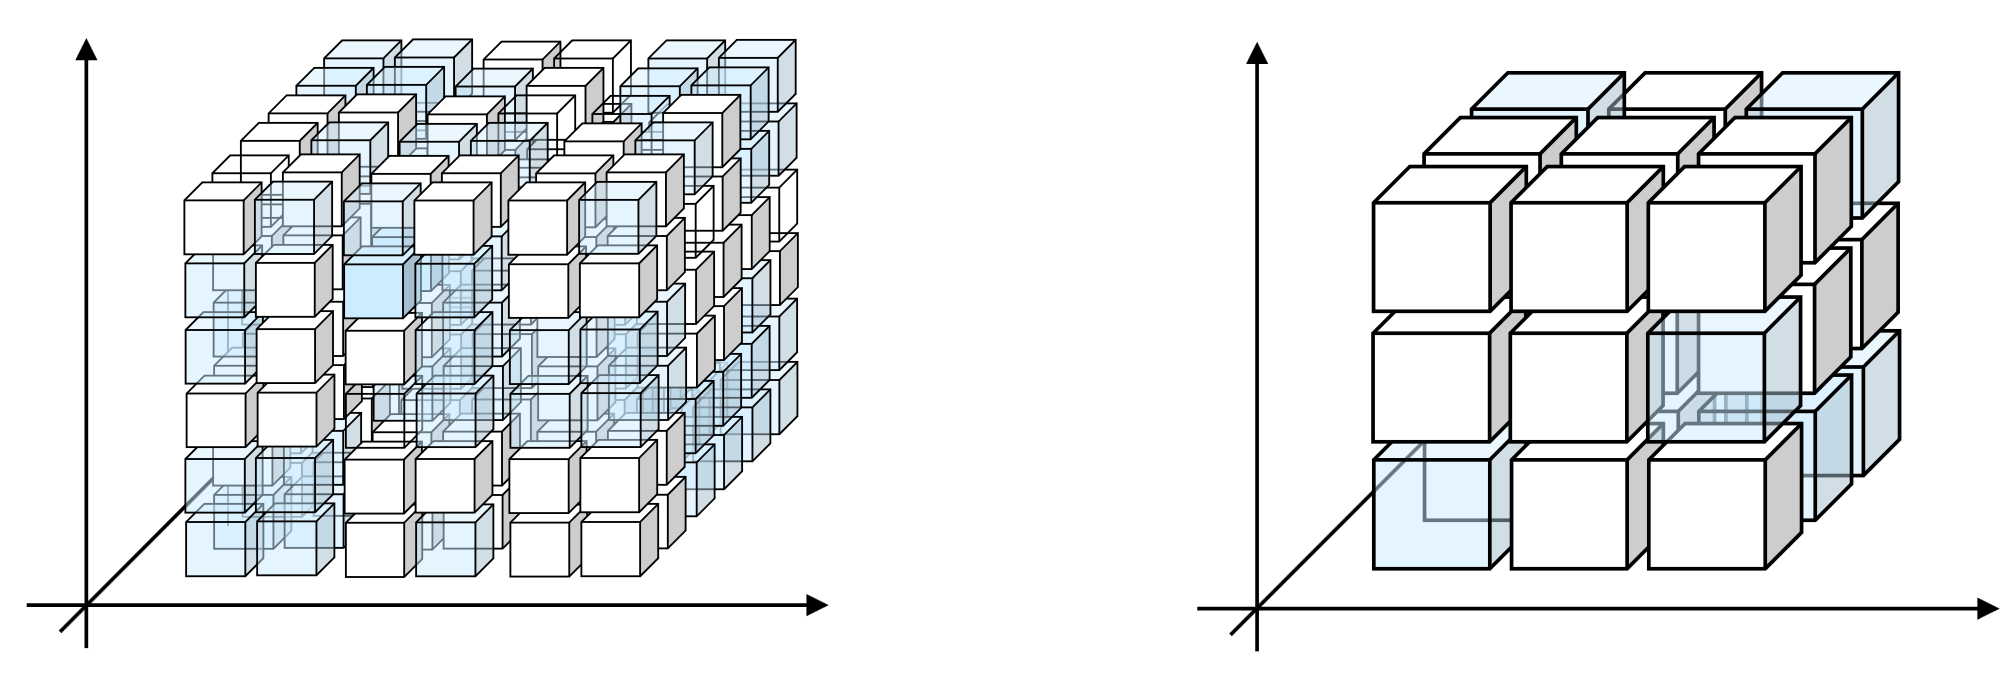
\includegraphics[width=0.7\textwidth]{capitoli/03_Data warehouse_progettazione concettuale e logica/images/sparsita.png}
    \caption{Esempio di sparsità dei dati: la matrice teorica (a sinistra) mostra tutte le combinazioni possibili, mentre la matrice reale (a destra) evidenzia solo le combinazioni effettivamente verificatesi.}
    \label{fig:sparsita}
\end{figure}

\section{Progettazione Logica: Il Modello Relazionale per il Data Warehouse}

La progettazione logica produce uno \textbf{schema logico relazionale (ROLAP)} partendo dal modello concettuale DFM. Si basa su due princìpi opposti rispetto ai database tradizionali:
1. Denormalizzazione delle tabelle.
2. Tolleranza (e ricerca) della ridondanza dei dati per ottimizzare i tempi di lettura.

\subsection{Lo Schema a Stella (Star Schema)}
È l'architettura standard per i data warehouse relazionali.
\begin{itemize}
    \item \textbf{Tabelle delle Dimensioni:} Si crea \textit{una sola tabella per dimensione}. Le gerarchie vengono schiacciate e perse a livello strutturale: gli attributi di diverso livello (es. Data, Mese, Anno) diventano colonne della medesima tabella, generando forte ridondanza (es. il mese e l'anno saranno ripetuti identici per ogni giorno di quel mese).
    La \textbf{Chiave Primaria} della tabella dimensionale è sempre una chiave generata artificialmente (\textbf{chiave surrogata}, un contatore intero), mai una stringa o una logica di business, per velocizzare le operazioni di \texttt{JOIN}.
    \item \textbf{Tabella dei Fatti:} Si crea al centro dello schema. Contiene come chiavi esterne le chiavi surrogate delle dimensioni e, come attributi diretti, tutte le misure.
\end{itemize}

% FIGURA ORIGINALE DA RECUPERARE DALLE SLIDE
% Slide di provenienza: 34
% Tipo: diagramma ER
% Descrizione: Diagramma E-R che mostra la struttura di uno Star Schema (Fatto al centro, Dimensioni intorno).
% Punto di inserimento: Qui, per illustrare lo Schema a Stella.
% File da inserire: star_schema.png
\begin{figure}[H]
    \centering
    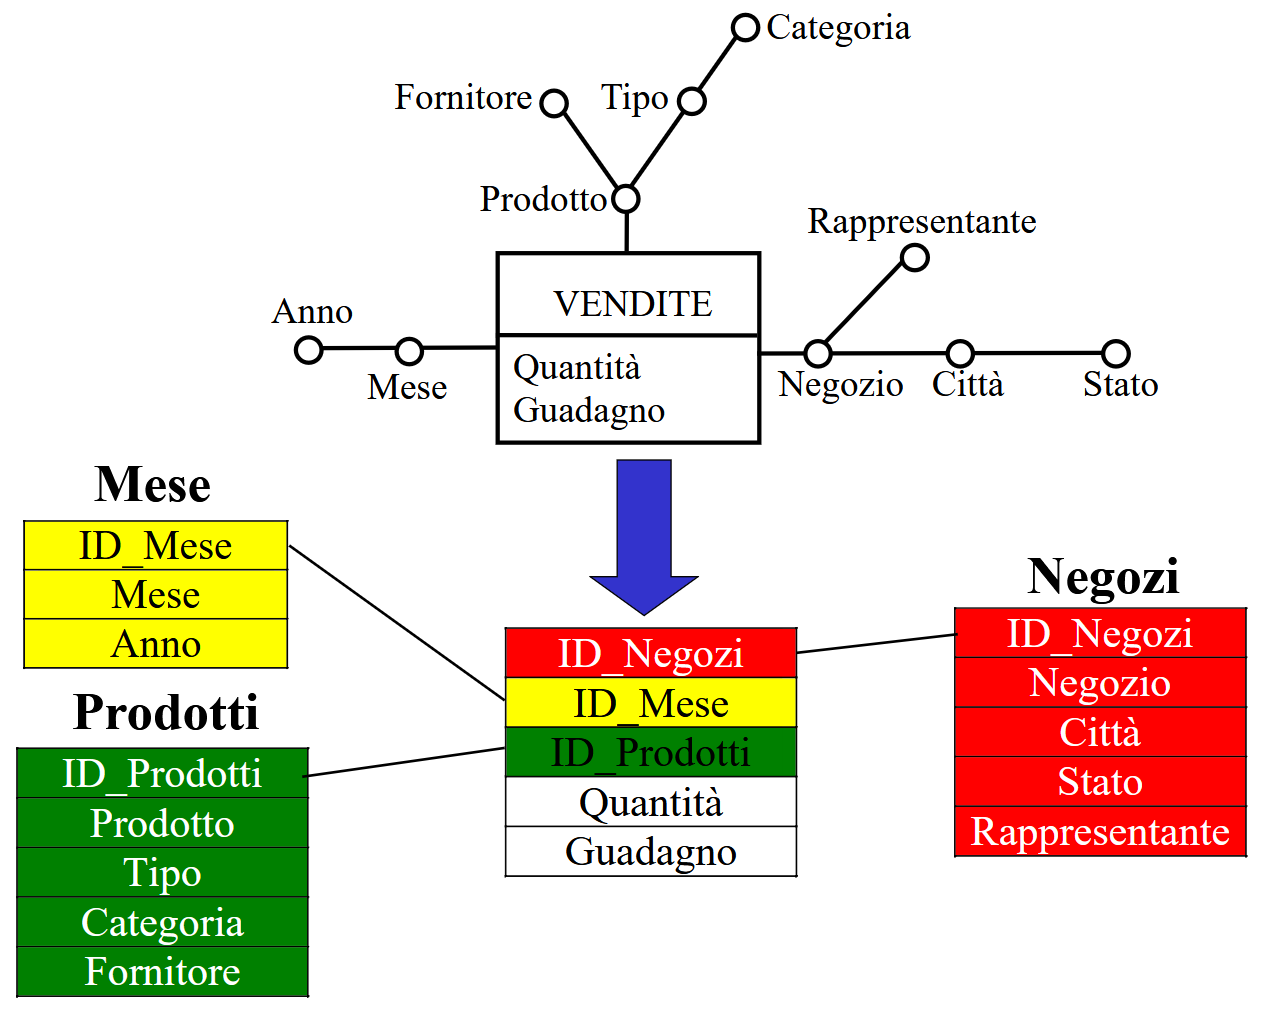
\includegraphics[width=0.75\textwidth]{capitoli/03_Data warehouse_progettazione concettuale e logica/images/star_schema.png}
    \caption{Struttura di uno Schema a Stella (Star Schema): il fatto centrale è circondato da tabelle dimensionali completamente denormalizzate.}
    \label{fig:star-schema}
\end{figure}

\subsection{Lo Schema a Fiocco di Neve (Snowflake Schema)}
Lo \textit{Snowflake Schema} tenta di reinserire la normalizzazione nello Star Schema. Sostanzialmente, si "taglia" una gerarchia dimensionale mettendola in una tabella separata (es. separando la gerarchia geografica dalla tabella Negozio).
\begin{itemize}
    \item \textbf{Difetti:} Il risparmio di spazio su disco è marginale (perché le tabelle dimensionali sono trascurabili rispetto ai milioni di record della tabella dei fatti). In compenso, per ricostruire l'informazione il sistema dovrà eseguire \texttt{JOIN} aggiuntivi, degradando le prestazioni.
    \item \textbf{Uso reale:} Lo schema Snowflake è fortemente sconsigliato e raramente utilizzato nella pratica aziendale.
\end{itemize}

\begin{figure}[H]
    \centering
    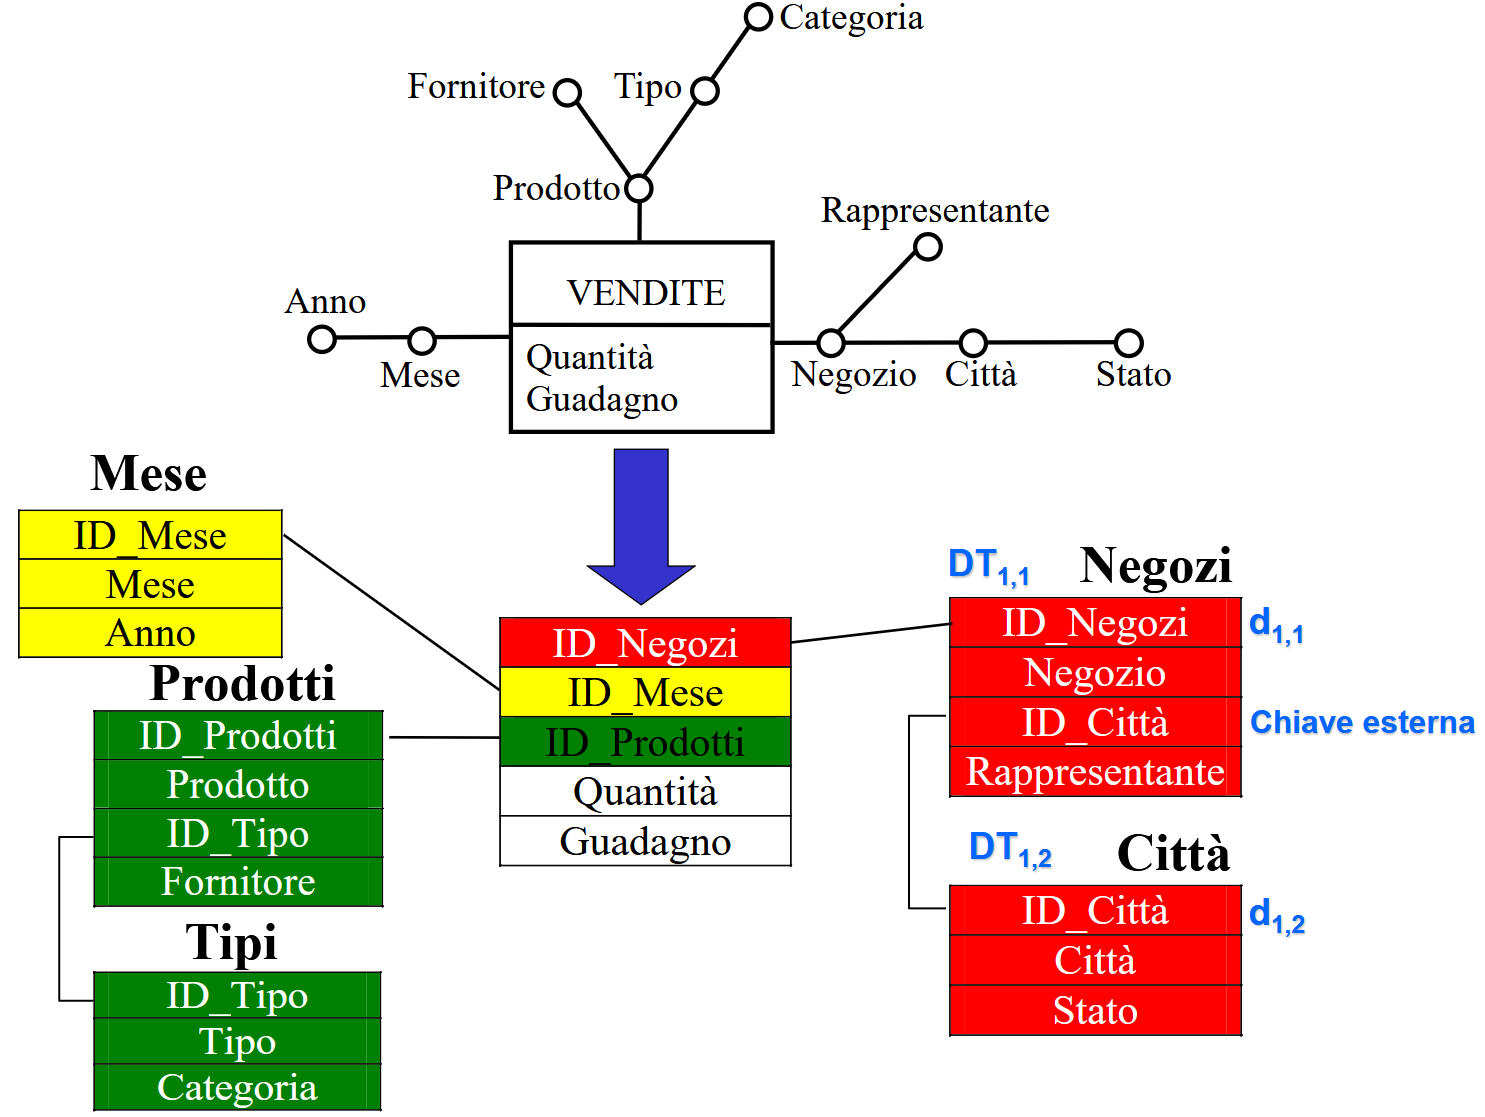
\includegraphics[width=0.75\textwidth]{capitoli/03_Data warehouse_progettazione concettuale e logica/images/snowflake_schema.png}
    \caption{Struttura di uno Schema a Fiocco di Neve (Snowflake Schema): la gerarchia geografica è separata dalla tabella Negozio, richiedendo un join aggiuntivo per ricostruire l'informazione.}
    \label{fig:snowflake-schema}
\end{figure}

\subsection{Traduzione Logica degli Archi Multipli}
Come si mappa l'arco multiplo (relazione N:M tra dimensioni) in un database relazionale? Esistono due soluzioni principali (oltre a quella dell'attributo configurazione già discussa):

\begin{enumerate}
    \item \textbf{Bridge Table (Tabella Ponte):} È la soluzione più ortodossa. Si crea una tabella intermedia tra il Fatto e la Dimensione multiautore (es. tra Vendita Libro e Autore). Questa tabella modella le coppie valide e introduce un \textbf{Peso} (es. 0.5 se gli autori sono due).
    \begin{itemize}
        \item \textit{Pro:} Permette interrogazioni pesate corrette (es. dividere l'incasso del libro equamente tra gli autori: \texttt{SUM(Incasso * Peso)}).
        \item \textit{Contro:} Rende complesse le query di semplice impatto (es. "Quante copie ha venduto l'autore in totale, a prescindere dal co-autoraggio?") e introduce un overhead di join.
    \end{itemize}
    \item \textbf{Push Down:} L'arco multiplo viene "spinto" direttamente nella Tabella dei Fatti. Il Fatto viene sdoppiato/moltiplicato: se un libro ha 3 autori, si creano 3 record nella tabella dei fatti, ognuno puntante a un autore diverso.
    \begin{itemize}
        \item \textit{Pro:} Costo di interrogazione bassissimo (elimina il join aggiuntivo).
        \item \textit{Contro:} Moltiplica enormemente lo spazio occupato dalla Tabella dei Fatti (che è già enorme). L'incasso andrebbe pre-frazionato (calcolato) durante la fase di ETL prima dell'inserimento, rendendo difficili eventuali variazioni. Le interrogazioni "di impatto" (senza frazionamento) diventano molto pericolose per il rischio di doppie somme.
    \end{itemize}
\end{enumerate}

\begin{figure}[H]
    \centering
    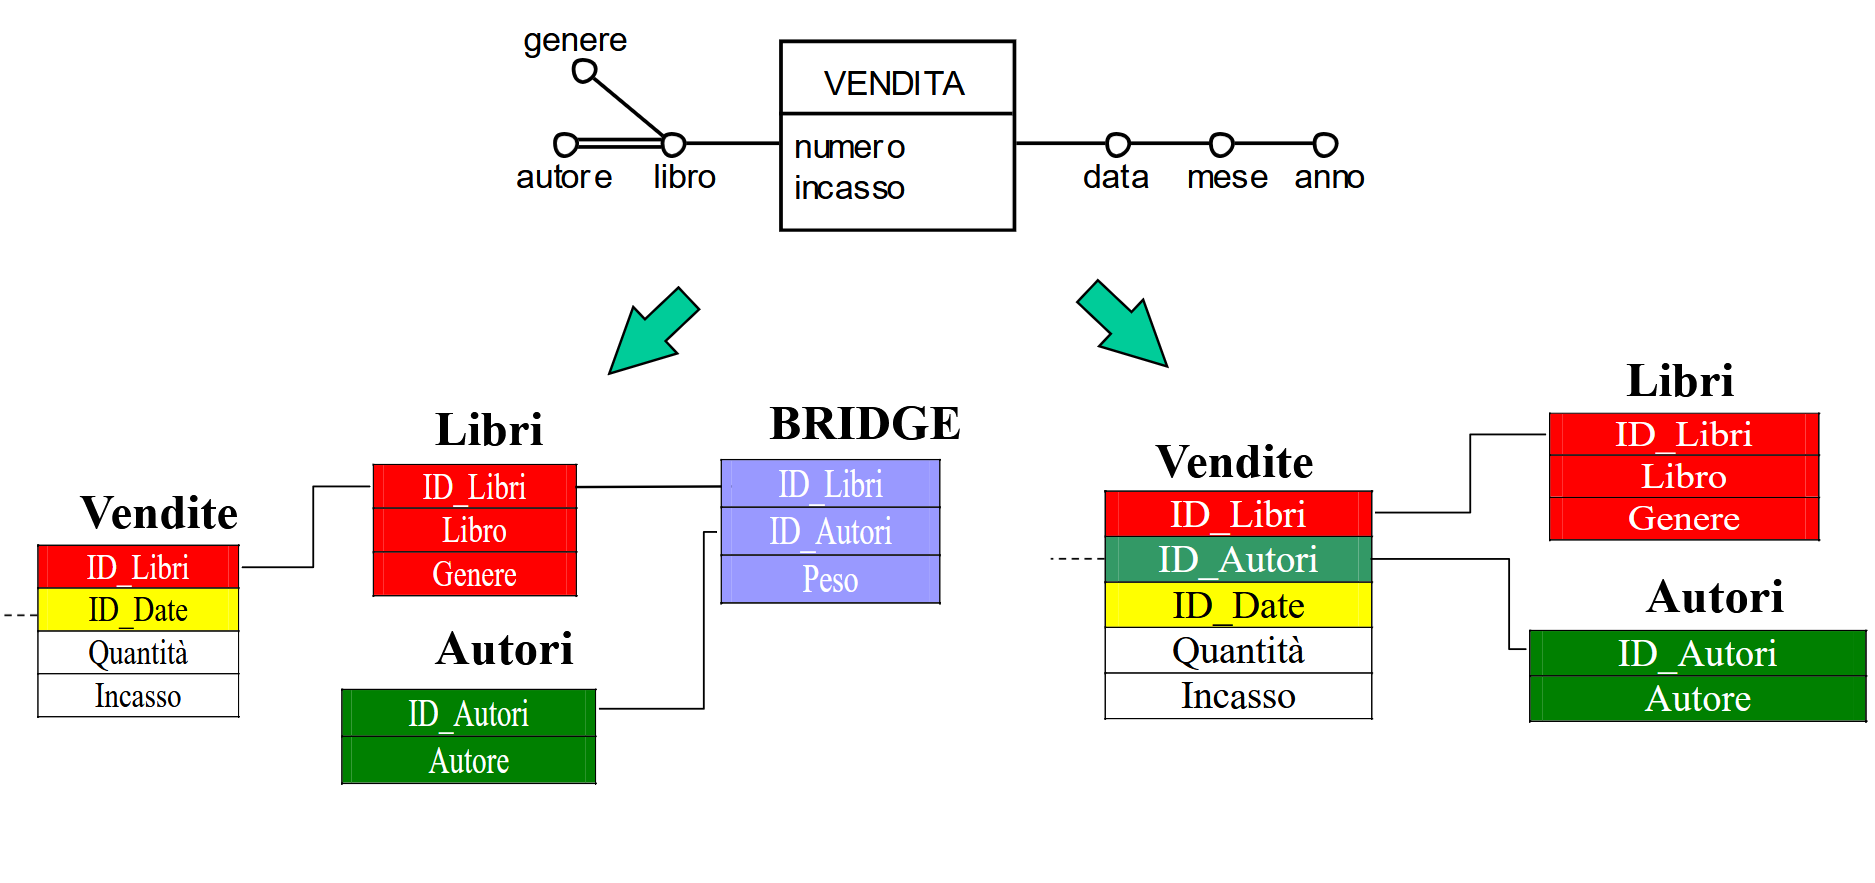
\includegraphics[width=0.75\textwidth]{capitoli/03_Data warehouse_progettazione concettuale e logica/images/archi_multipli.png}
    \caption{Traduzione logica di un arco multiplo: a sinistra la soluzione con Bridge Table, a destra la soluzione Push Down.}
    \label{fig:archi-multipli}
\end{figure}

\subsection{Dimensioni Degeneri e Junk Dimension}
Una dimensione è \textit{degenere} quando, dopo l'analisi, risulta composta da un \textbf{solo attributo} (privo di gerarchie). 
Per mappare queste dimensioni logicamente, esistono due vie:
\begin{enumerate}
    \item \textbf{Integrazione nella Tabella dei Fatti:} (Push down). L'attributo viene inserito come normale colonna all'interno del Fatto, senza creare una tabella dimensionale esterna.
    \item \textbf{Junk Dimension (Dimensione "pattumiera"):} Se ci sono molte dimensioni degeneri scorrelate (es. flag di stato, tipi di spedizione, codici semplici), le si compatta tutte in un'unica dimensione artificiale che contiene il \textit{prodotto cartesiano} di tutte le combinazioni possibili di questi attributi. Nella tabella dei fatti risiederà solo un ID puntatore a questa riga. Questa soluzione è adottabile solo se la cardinalità risultante (le combinazioni totali) rimane piccola.
\end{enumerate}


\begin{figure}
    \centering
    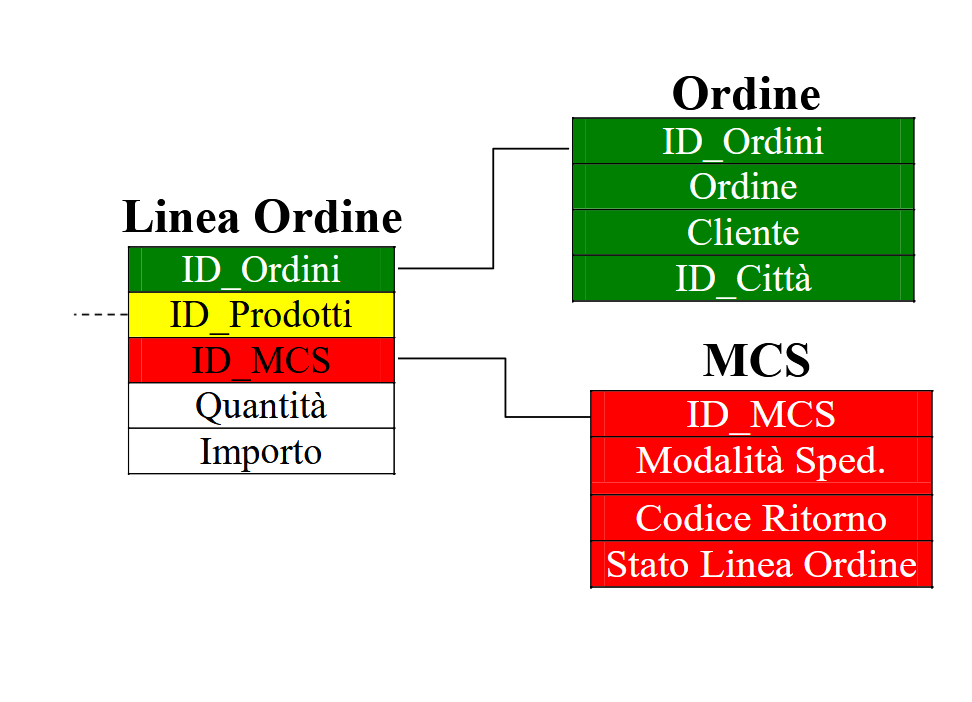
\includegraphics[width=0.75\textwidth]{capitoli/03_Data warehouse_progettazione concettuale e logica/images/junk_dimension.png}
    \caption{Esempio di Junk Dimension: le dimensioni degeneri "Tipo Spedizione" e "Flag Stato" vengono combinate in un'unica tabella dimensionale, riducendo il numero di join nella Tabella dei Fatti.}
    \label{fig:junk-dimension}
\end{figure}
% ==============================================================================
% FINE DISPENSA
% ==============================================================================